\documentclass{article}

% if you need to pass options to natbib, use, e.g.:
%     \PassOptionsToPackage{numbers, compress}{natbib}
% before loading neurips_2021

% ready for submission
\usepackage[preprint]{neurips_2021}

% to compile a preprint version, e.g., for submission to arXiv, add add the
% [preprint] option:
%     \usepackage[preprint]{neurips_2021}

% to compile a camera-ready version, add the [final] option, e.g.:
%     \usepackage[final]{neurips_2021}

% to avoid loading the natbib package, add option nonatbib:
%    \usepackage[nonatbib]{neurips_2021}

\usepackage[utf8]{inputenc} % allow utf-8 input
\usepackage[T1]{fontenc}    % use 8-bit T1 fonts
\usepackage[colorlinks=true]{hyperref}       % hyperlinks
\usepackage{url}            % simple URL typesetting
\usepackage{booktabs}       % professional-quality tables
\usepackage{amsfonts}       % blackboard math symbols
\usepackage{nicefrac}       % compact symbols for 1/2, etc.
\usepackage{microtype}      % microtypography
\usepackage{xcolor}         % colors
\usepackage{graphicx,subfigure}
\title{Transport time analysis of Tübingen}


% The \author macro works with any number of authors. There are two commands
% used to separate the names and addresses of multiple authors: \And and \AND.
%
% Using \And between authors leaves it to LaTeX to determine where to break the
% lines. Using \AND forces a line break at that point. So, if LaTeX puts 3 of 4
% authors names on the first line, and the last on the second line, try using
% \AND instead of \And before the third author name.

\author{%
  Frederic Becker\\
  \texttt{\small Matrikelnummer 4082451 }\\
  \texttt{\scriptsize frederic.becker@student.uni-tuebingen.de} \\
  \And
  Jan-Niklas Dihlmann\\
  \texttt{\small Matrikelnummer 4117847}\\
  \texttt{\scriptsize jan-niklas.dihlmann@student.uni-tuebingen.de} \\
}

\begin{document}

\maketitle

\begin{abstract}
   Every day a large number of people decide which mean of transport to pick to reach a certain destination. To compare the travel times of driving, bicycling and walking in the city of Tübingen, we created a pipeline for creating isochrone maps querying the Google Maps API. This special map visualizes travel times for a route that goes from a specific starting point to any location on the map. In addition, we regressed travel times with a linear regression model based on horizontal and vertical distances between the starting and destination location. We found that the isochrone maps captured a salient traffic characteristic of Tübingen and that bicycling is a good alternative for driving, in case no hills have to be climbed. However, our work is limited to a single starting location in Tübingen.  
\end{abstract}

\begin{center}
    \href{https://github.com/JDihlmann/isomap}{Github Repository: Isomap} 
\end{center}

\section{Introduction}
% Topic introduction --> all keywords
% isochrone maps --> description and related work
Every day, billions of people use different modes of transportation to get to work, school or university. Travel time usually depends on the choice of transport, the distance of the route, the traffic situation and, in some cases, even the weather conditions. Nevertheless, route planning services such as Google Maps \cite{googleMaps} manage to provide reliable estimates of travel time. Isochrone maps show how travel times evolve in the environment. More specifically they display the travel time required to get from a fixed starting point to locations on the map. This visualization of location-dependent travel times is particularly useful for identifying anomalies and large shifts within travel times. For example this publicly available map \cite{redditMap} displays the minimum travel time from Paris to any place in France for bike, train and car. 

% Erklären wieso wir einen Regressor haben (Kosten / Testen ob funktioniert)
% Our work isochrone % Our work regression
In this report, we will describe our approach of creating an isochrone map for the city area of Tübingen, Germany considering travel times by foot, bike and car. This process consisted of three steps: First, we created a grid of locations depicting the area of Tübingen. Second, we queried the Google Maps API for travel times and elevation data. Third, we visualized the obtained data in an isochrone map. In addition, we regressed travel times with a linear model to identify possible salient differences between the means of transportation and to test to which extent travel times within Tübingen can be predicted by the horizontal and vertical distance between the start and destination of a route.

% Report outline
In the next section we will describe our data collection scheme. In section 2 we will present the isochrone maps and the regression results. In the last section we will summarize and conclude. 

\section{Data collection and mapping}
% general frame
We developed a data collection pipeline to query samples of travel time from an arbitrary location of origin and a corresponding region of destinations. This pipeline receives a location of origin and queries samples of travel time in a destination grid, that can be specified in sampling rate, bound size and transportation type. For the instance of Tübingen we specified the origin as the \textit{Tübingen Rathaus} with coordinates~$(\text{Lat: } 48.5204497, \text{Lng: } 9.0534181)$ and the region of destinations as a squared surrounding area of~$16 \text{km}^2$ in size sampled by~$1600$ evenly arranged grid points. 

% Querying
To obtain estimated travel times we queried the Google Maps Distance API \cite{googleMapsDirectionsAPI} for walking, bicycling and driving. It is import to note, that the Google API moves destinations that are not reachable by the specified mean of transport to the nearest reachable position. As a consequence, the final sample locations differed between transportation types even tough the same destination grid was queried. We stored the entire JSON retrieved from the Google API including directions, bounds and most importantly duration. Finally we obtained a dataset with~$1600$ samples per transportation type and ~$2573$ unique locations. To provide the regression analysis with vertical distances, we additionally created a pipeline for the Google Maps Elevation API \cite{googleMapsElevationAPI} to query and store the elevation for each individual site in our dataset. Since the Google API is costly and we used up our free contingent it was not possible to increase the sample size.

% Map construction
To create the isochrone maps we divided the range of travel times into $10$ equally sized bins and then plotted the contours of the corresponding locations within a bin which defined regions that can be reached in similar time from the starting position. This visualization corresponds to the definition of an isochrone map. The elevation map was constructed in a similar fashion, whereby we additionally highlighted locations that are below the origin location with dots. 

%In order to create an isochrone map as well as a regressor for it, we need to collect samples of travel time from an arbitrary origin point and a corresponding region.In order to do so we developed a flexible data collection pipeline, that receives an origin point and queries samples of travel time in a grid, that can be specified in sampling rate, bound size and transportation type. 

%For the instance of Tübingen we specified the origin as the \textit{Tübingen Rathaus} with coordinates~$(\text{Lat: } 48.5204497, \text{Lng: } 9.0534181)$ and the region of destinations as a squared surrounding area of~$16 \text{km}^2$ in size sampled by ~$1600$ uniformly distributed points.In order to retrieve the travel time we query the Google Maps Distance API \cite{googleMapsDirectionsAPI} for the transportation types walking, bicycling and driving. It is import to note, that although we query the Google API with a coordinate grid, the Google API will automatically move the point to the nearest reachable position, thus sample positions for each transportation type might differ, since some places aren't reachable with a car or a bike. We store the entire JSON we retrieve from Google Maps, with directions, bounds and most importantly the duration. This results in a final data set of~$1600$ samples for each transportation type, with a total of~$2573$ unique locations, due to the automatic movement. Additionally we build a small pipeline to query the Google Maps Elevation API \cite{googleMapsElevationAPI}. For the isochrone map of Tübingne we queried all~$2573$ unique locations and stored the elevation of each point as well. Although we do not think that it would be necessary but we weren't able to increase the sample size further since the Google API is costly and we used up our free contingent.

\section{Isochrone Maps}
% \item Visualisation (Maps for each transportation / Difference maps)
% \item Regression results
% \item Compare regressor from Tuebingen to Heidelberg

% motivation --> maybe move to introduction
Isochrone maps are an elegant tool for visualizing travel times for a route that goes from a specific starting point to any location on the map. It provides an intuitive way to analyze the differences in transportation time between different modes of transportation and helps to find bottlenecks in the underlying city structure and the corresponding traffic system. This is especially interesting for Tübingen, as there is always a debate which transportation is the fastest. Tübingen is also known as a large one-way street for cars, so it will be interesting to see if this is reflected in the corresponding isochrone map. 

% description of results
The isochrone maps for walking, bicycling and driving are presented in Figure \ref{fig:maps}a-c. The isochrone map for walking forms a radial pattern spreading from the origin point more or less evenly in all directions. The inner city can be reached within 8 minutes and the margins of the map within 80 minutes. The isochrone map for bicycling is more irregular structured. The contours are more elongated and extend parallel to the river Neckar. Using the bike, the inner city can be reached within 4 minutes and the margins of the map within 36 minutes. The isochrone map for driving is similar to bicycling map. Interestingly, the map includes single blobs of high travel times that are not part of the other maps and which represent most-likely areas like woods in which driving is not possible. By car the inner city can be reached within 6 minutes and the margins of the map within 27 minutes.

% interesting points
Locations near the origin are faster reachable by foot and by bike than by car. This is because the starting point is near the historic center of Tübingen, which is closed to cars, therefore Google Maps suggests a large detour for this area. In addition, destinations along the eastern riverbed appear to be difficult to reach by car. This area fits very well with the Gartenstraße which is fastest to reach via a one-way street in the direction of the historic center, which results in a long detour for cars. Furthermore, the same one-way street crosses the Neckar and connects the lower and upper city centers. According to the isochrone maps, the lower city center is quicker to reach by foot and by bicycle than by car. The isochrone maps can thus capture and depict a prominent traffic architecture of Tübingen very well.

%As stated before an isochron map is an elegant tool to visualize the travel time from a specific origin. With it is easy to analyze transportation time differences by means of transportation. We thus can compare which modes of transportation are more efficient than others and also find bottlenecks in the underlying city / traffic system. This is especially interesting for Tübingen, as there is always a debate which transportation is the fastest. It also should be noted that Tübingen is known as big one-way street for cars, therefore it is interesting to see if this is also visible in the corresponding isochrone map. 
% construction
%The isochrone maps [\ref{fig:maps}] of Tübingen were generated with the data acquired from the Google API. For each transportation type we divided the full range of travel time into $10$ equally sized steps. We then plotted the contours of those steps, resulting in regions of travel time fitting the definition of an isochrone map. The elevation map was constructed in a similar fashion, we additionally plotted the sample points that are below the origin location.  

% interpretation & comparison
%Looking at the result of the isochrone maps of Tübingen and comparing them, it is interesting to see that they all differ from each other. While the walking map does almost form a radial pattern, the bicycling map is stretched along the river and the driving map has lots of patches. The car map also has certain part that are not reachable. Comparing the driving and bicycling maps by duration, it is visible that some points that are near the origin are faster reachable by bike than by car. Most of this points lie in the north east of the origin and are those points that are on the other side of the Neckar, the river that flows through Tübingen. There are even some points that are faster reachable by foot than by car, these points have a similar position to those that are faster reachable by bike. It thus can be stated, that if one wants to reach the other side of the river fast, it will be better to walk or to take the bike. 

% TODO: Finish textSpeculating on those results one could start comparing the    

\begin{figure}
  \centering
  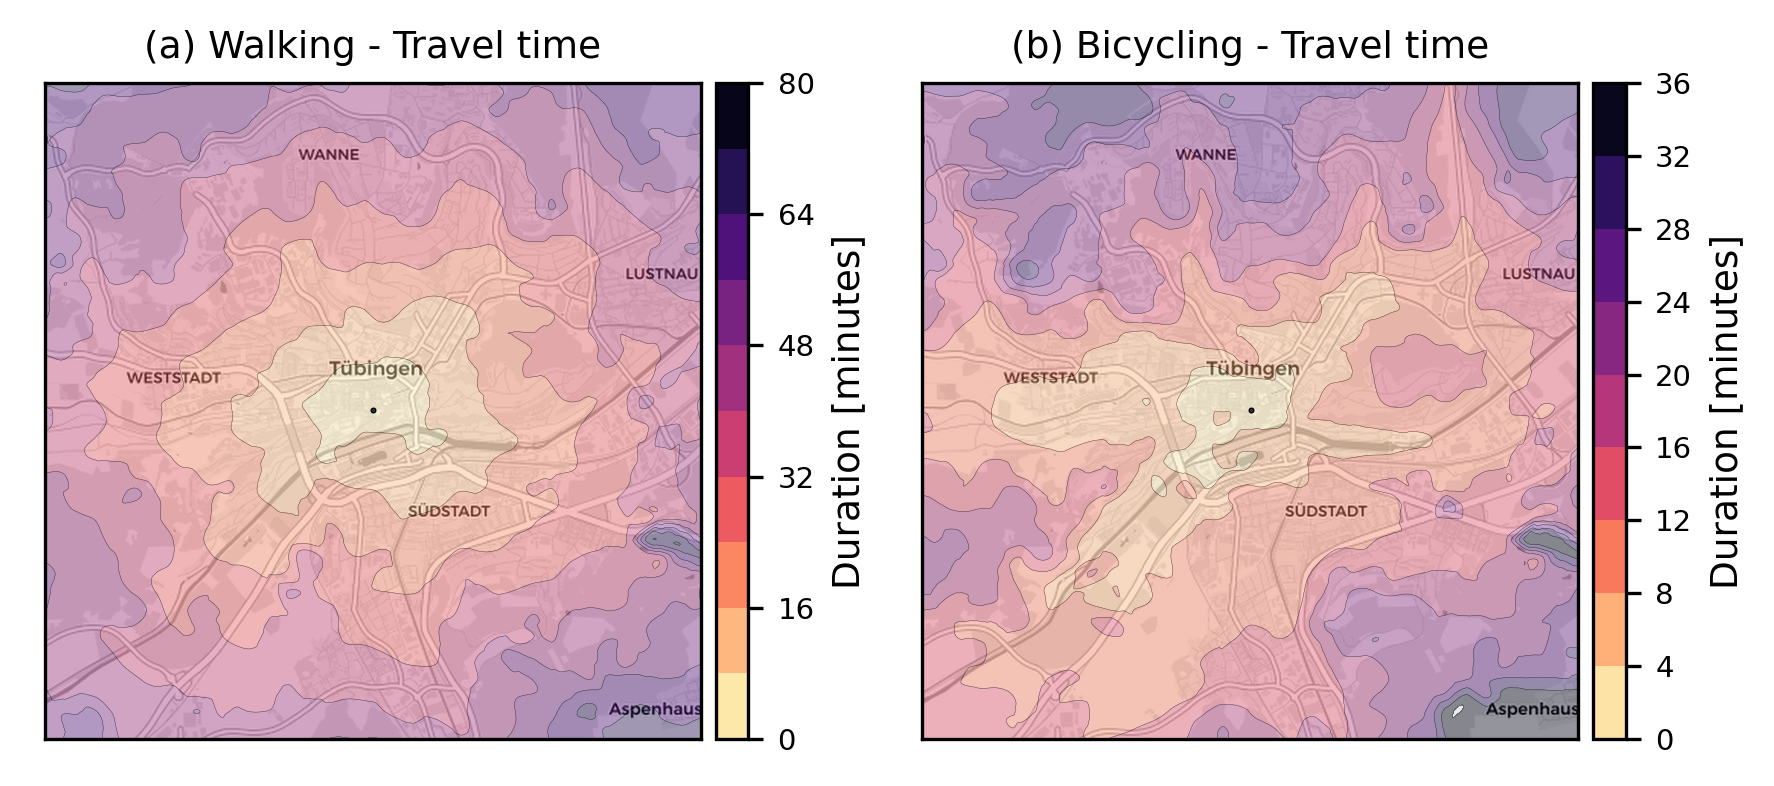
\includegraphics[width=\linewidth]{fig/RegionDisplayer_WalkingBicycling.png}
  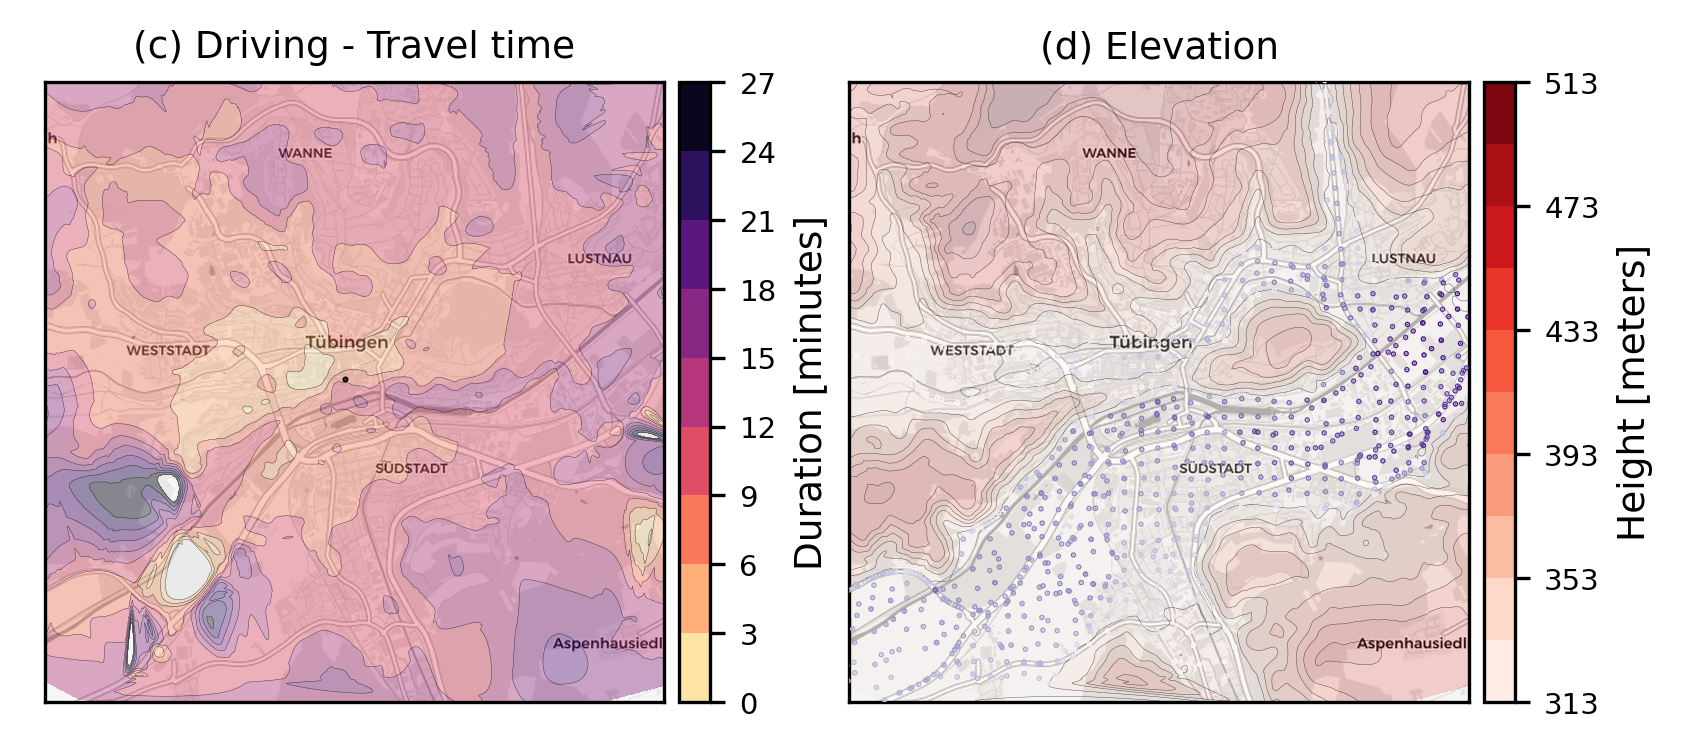
\includegraphics[width=\linewidth]{fig/RegionDisplayer_DrivingElevation.png}
  \caption{Isochrone maps (a,b,c) and elevation map (d) of the city Tübingen, Germany. The black dot in the isochrone maps denotes the origin point, which is the Tübingen Rathaus. Each other location on the map is color coded indicating the time (in minutes) it takes traveling to that specific location. The elevation map shows the relative height (in meters). Additional points indicate regions that are lower than the origin (darker equals lower).}
  \label{fig:maps}
\end{figure}

\section{Regression Analysis}

% motivation
The travel time algorithm underlying the Google Maps API is not publicly available. Still, it can be assumed that it integrates a variety of datapoints on traffic, distance and past user travel times in a A* fashion algorithm. The aim of our analysis was to test to what degree this travel time calculation can be approximated by two rather simple predictors namely the horizontal and vertical distance between the starting and the ending location of the route and to describe the differences in travel time between the different means of transportation numerically.

% model types % model formula
We fitted two additive linear models to regress travel time each considering different predictor variables. The horizontal model $M_h$ only included the horizontal distance between the origin and the destination as predictor. The combined model $M_{hv}$ additionally included the absolute vertical distance between the origin and the destination as predictor: travel time \raisebox{-0.9ex}{\~{}} horizontalDistance + verticalDistance. We chose an additive model formulation that estimates the speed differences between driving, bicycling and walking per predictor explicitly. In addition, we constraint the model to have an intercept of zero as it does not require any time to reach one's own position. Travel time was given in seconds and distances in meter. The combined model achieved a lower mean absolute error ($M_{hv}$: 2.5 min, $M_{h}$: 3.4 min) and a lower BIC value than the horizontal model ($M_{hv}$: 64566, $M_{h}$: 67315). The combined model thus explains the data better and is able to regress travel times with a average deviation of 16\%. 

\begin{figure}[h]
  \centering
  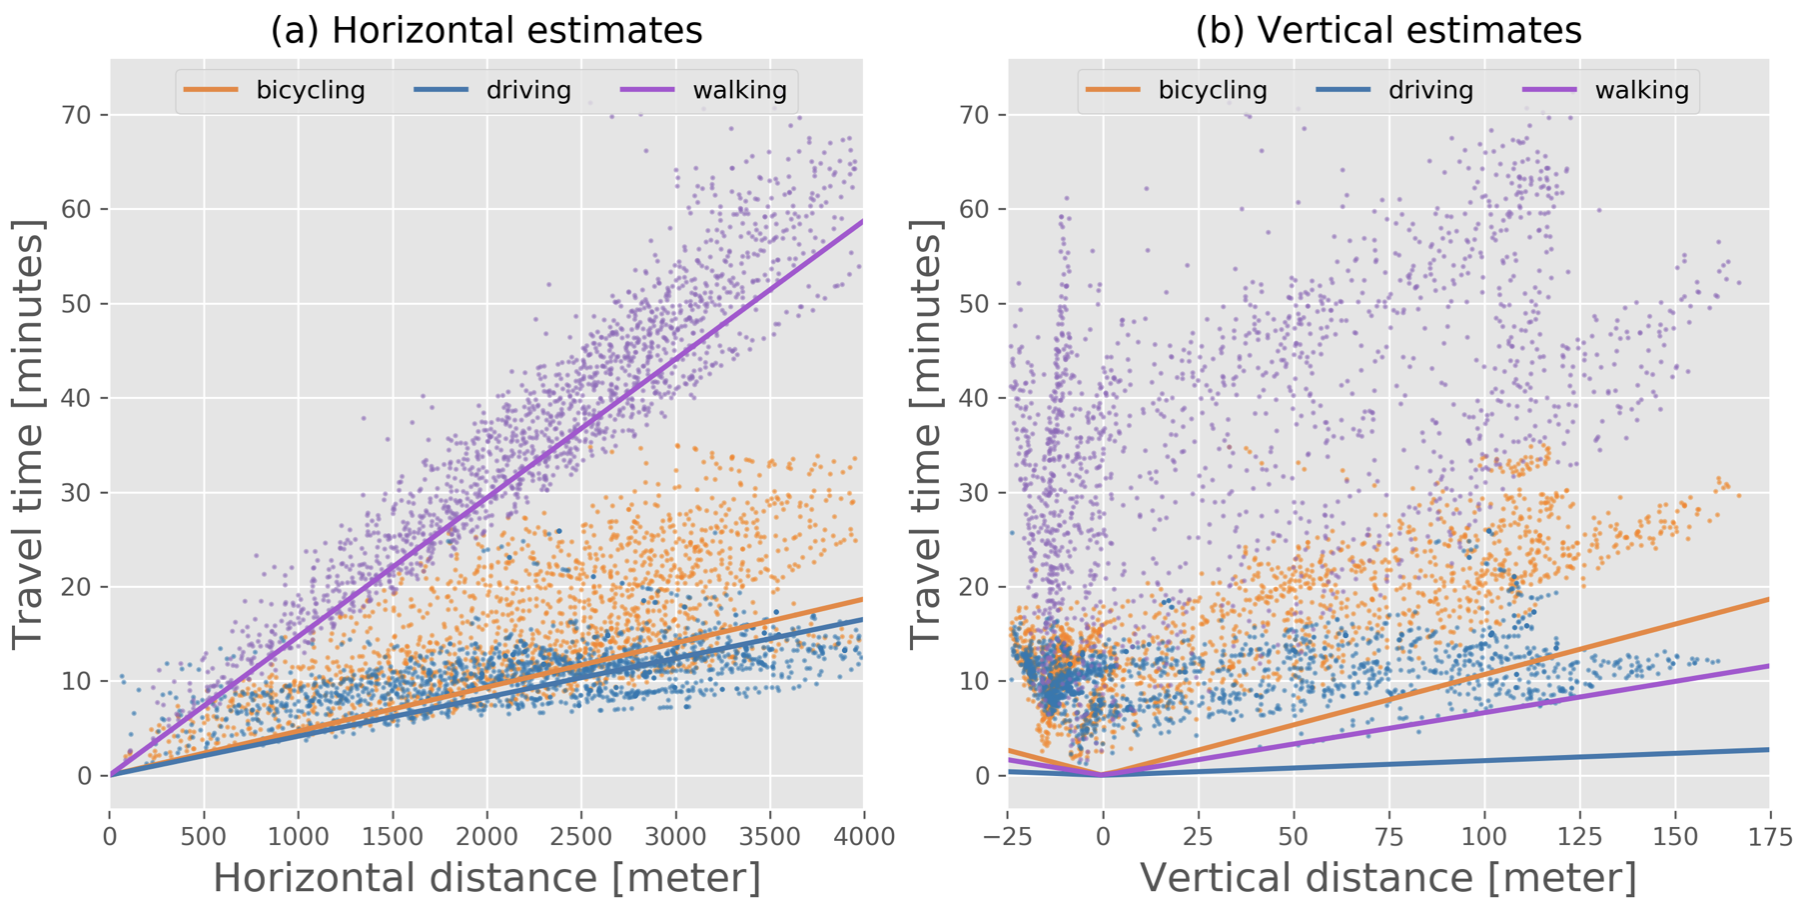
\includegraphics[width=\linewidth]{fig/RegressionPlots_CombinedEstimates.png}
  \caption{Regression of travel times in Tübingen. Fits of the combined model presented for driving, bicycling and walking per predictor variable i.e. horizontal distances (a) and vertical distances (b). Confidence intervals of the regression lines were omitted as they are too narrow to illustrate.}
  \label{fig:regression}
\end{figure}

% result + interpretation 
The combined model estimates that a car travels horizontal distances at 17 km/h ($\beta = 0.25, $ CI $=[0.24, 0.25], p<.001$), a bicycle slower at 12.8 km/h ($\beta = 0.03, $ CI $=[0.02, 0.04], p<.001$), and a pedestrian significantly slower at 4 km/h ($\beta = 0.60, $ CI $=[0.59, 0.61], p<.001$), as illustrated in Figure \ref{fig:regression}a. Thus bicycling is only slower to an extent of approximately 4 km/h given a flat route. The different velocities are also reflected in the different time scales of the isochrone maps (see Fig.~\ref{fig:maps}). Vertical distances are traveled with a speed of 2 km/h ($\beta = 0.93, $ CI $=[0.69, 1.18], p<.001$) by car (see Fig. \ref{fig:regression}b). Significantly slower is the bike with 0.6 km/h ($\beta = 5.47, $ CI $=[5.13, 5.82], p<.001$), whereas walking is significantly faster than bicycling with 1 km/h ($\beta = -2.43, $ CI $=[-2.77, -2.08], p<.001$). The car is slowed down by vertical distances by a factor of 8.7, the bike by a factor of 22.5 and the pedestrian only by a factor of 4.2. This resembles very nicely that walking is relatively insensitive to the topology which is mirrored by the radial pattern in the isochrone map for walking, whereas the isochrone maps for driving and bicycling are more shaped by the topology. Furthermore, the estimates imply that bicycling is a serious alternative to driving as long as no major vertical distances have to be climbed. This corresponds very well to the fact that people bicycle less frequently in hilly cities than in flat cities \cite{bic}.

\section{Conclusion}
We presented a pipeline for creating isochrone map for arbitrary locations. and demonstrated it at the example of Tübingen. The presented isochrone maps were able to capture basic traffic characteristics of Tübingen, in addition the analogous regression analysis of travel times suggested that bicycling is a good alternative to driving but forfeits if vertical distances have to be traveled whereas walking is pretty insensitive to vertical distances. However our results are very limited. First, all our results rely heavily on the accuracy of Google's travel time computation. Second, our analysis is only valid for the specific starting location and may differ for other starting locations and cities.


% Nur Stichpunktartige Gedanken
%Isochronmaps are a great tool to visualize traffic and find interesting structure in the dynamics of a city
%Our pipeline can bes used to generate isochronemaps at differnt times of day ... finding causes for traffic jams
%It also can be used to recommend different modes of transportation, for Tübingen for example many points can be reached faster by bike than by driving. 

% Amerkungen Treffen 
% Erklären wieso wir einen Regressor haben (Kosten / Testen ob funktioniert)
% Fokus ist Bericht gut schreiben und Sachen von VL benutzten (Haben wir Statistische Analyse)
% Evtl. bei Regressor mehr Variablen und am Ende sagen das die aktuellen schon reichen 
% Evtl mit anderer Stadt vergleichen

\bibliographystyle{alpha}
\bibliography{bibliography}


% model formula
%We fitted three different regression models for travel time each considering different predictor variables. The horizontal model $M_h$ only included the horizontal distance between the origin and the destination as predictor. The simple combined model $M_{hv}$ included additionally the absolute vertical distance between the origin and the destination as predictor. The extended combined model $M_{hv\pm}$, on the contrary, included uphill (origin is at lower elevation than destination) and downhill (origin is at higher elevation than destination) distances between the origin and the destination separately as predictor. Each model was formulated in a nested fashion. Distance$_{WBD}$ estimates the effect of distance on travel times for driving. Distance$_{WB}$ estimates the effect of distance on travel times for bicycling compared to driving. Distance$_{W}$ estimates the effect of distance on travel times for walking compared to bicycling. We chose this formulation to estimate the differences between driving, bicycling and walking explicitly. In addition, we constraint the model to have an intercept of zero as it does not require any time to reach one's own position. Travel time was given in seconds and distances in meter. 


% model comparison
%The simple combined model achieved a lower mean absolute error ($M_{hv}$: 2.5 min, $M_{h}$: 3.4 min) and a lower BIC value than the horizontal model ($M_{hv}$: 64566, $M_{h}$: 67315). Thus, absolute vertical distances have predictive power for estimating travel times. The extended combined model achieved a lower mean absolute error ($M_{hv+}$: 2.4 min) and a lower BIC score than the simple combined model ($M_{hv+}$: 64311). The extended combined model thus explains the data best and is able to regress travel times with an accuracy of 15\%. 

% reporting
%The extended combined model suggests that a car travels direct horizontal distances with 17.0 km/h ($\beta = 0.21, p<.001$). Bicycling is estimated significantly slower and achieves 12.8 km/h ($\beta = 0.07, p<.001$). Thus bicycling is only slower to an extent of approximately 4 km/h given a flat route in Tübingen. In comparison the model estimates walking speed to be 4 km/h which is significantly slower than bicycling and driving ($\beta = 0.61, p<.001$). Note that all speed estimations do not describe the actual movement speed but only the travel speed for horizontal or vertical beeline distances. 

%For vertical uphill distances the model estimates a car will travel 2 km/h ($\beta = 1.84, p<.001$). This is about 8.5 times slower than for horizontal distances. The uphill travel speed of a bicycle is 0.6 km/h which is significantly slower than driving ($\beta = 4.52, p<.001$). Interestingly, bicycling is slowed down by uphill distances in particular namely by a factor of 21.3. The model estimates the uphill walking speed to be 1 km/h which is significantly faster than bicycling ($\beta = -2.60, p<.001$) and 4 times slower than horizontal walking. Vertical downhill speed of a car is 0.3 km/h ($\beta = 14.39, p<.001$). For bicycling the speed is estimated to be 0.6 km/h ($\beta = -8.73, p<.001$) and for walking 5.9 km/h ($\beta = -5.06, p<.001$). Traveling downhill seems to be very costly for driving. Bicycling downhill or uphill does not make a difference. Walking downhill is faster than in flat or uphill routes.

% interpretation 



\end{document}
